\chapter{Related Work} \label{chapter:related-work}
Having introduced the historical underpinnings of our work and placed our experiments within context, we turn to a survey of the more recent literature, in an effort to demonstrate the research gaps that currently exist and how our work fills them. In particular, I will review current literature on uncertainty quantification and Bayesian reasoning in Large Language Models, notably focusing on the clinical domain and closed LLMs. 

\section{Definitions of Uncertainty in Machine Learning}
An adequate model of uncertainty is vital in healthcare applications. Despite advancements in explainable AI, LLMs are inherently black-box models, as their underlying decision-making process is largely nonlinear and complex. Therefore, it is important for models to have a consistent and accurate estimation of their own uncertainty. Due to the relatively recent emergence of the field of uncertainty quantification (UQ), it remains somewhat unstructured, with key definitions of uncertainty still subject to ongoing debate. Here, we adopt a definition of uncertainty from a recent review that addresses uncertainty at various stages of the neural network training/prediction pipeline. We will also distinguish the two main types of uncertainty: aleatoric and epistemic \citep{kiureghianAleatoryEpistemicDoes2009}. 

We first define a neural network as a non-linear function $f_{\theta}$ parameterized by network weights $\theta$ that maps a measureable input set $\mathbb{X}$ to a measureable set $\mathbb{Y}$ as such:

\begin{equation} \label{eq:nn}
f_{\theta}:\mathbb{X} \rightarrow \mathbb{Y} \qquad f_{\theta}(x) = y
\end{equation}

We can further define a training dataset in the supervised learning case:

\begin{equation} \label{eq:train-data}
\mathcal{D} = (\mathcal{X},\mathcal{Y}) = \{x_n, y_n\}_{n=1}^{N} \subseteq \mathbb{D}
\end{equation}

where $\mathcal{D} \subseteq \mathbb{D} = \mathcal{X} \times \mathcal{Y}$ and $N$ is the number of samples in the training set. A new data sample $x^{*} \in \mathbb{X}$, a neural network on $\mathcal{D}$ can be used to predict a corresponding target $f_{\theta}(x^{*})=y^{*}$. This can also be extended to zero-shot evaluation as the neural network (a black-box LLM in our case) is trained on $\mathcal{D}$ as the set of text in the English language. Given this definition, there are 4 places uncertainty can arise from: (1) the \emph{data acquisition} process, (2) the \emph{neural network building} process, (3) the \emph{applied inference} model, (4) the \emph{prediction's uncertainty} model. Uncertainties associated with (3) and (4) are differentiated by out-of-domain errors vs. errors caused by in-domain input data $x^{*}$ and the model $f_{\theta}$ \cite{gawlikowskiSurveyUncertaintyDeep2023}. 

We are mainly interested in the \emph{prediction's uncertainty} as we cannot control the other sources of uncertainty in a black box model and we mainly would like to evaluate uncertainty as a function of prediction to promote physician-AI collaboration. Therefore, we are mostly interested in the uncertainty of a prediction $y^{*}$. The Bayesian framework offers a solid basis for analyzing this uncertainty. We can consider the probability distribution for a prediction $y^{*}$, based on a sample input $x^{*}$ as:

\begin{equation} \label{eq:nn-posterior}
p(y^{*}|x^{*}) = \int_{D}{p(y^{*}|\mathcal{D},x^{*})}.
\end{equation}

We can also define a maximum a posteriori (MAP) estimation over the distribution of $y^{*}$ by:

\begin{equation}\label{eq:nn-map}
y^{*} = arg\ \max\limits_{y}\ p(y|x^{*}).
\end{equation}

Unfortunately, the distribution in \eqref{eq:nn-posterior} can only be approximated by the data given in $D$. We can decompose the probability of any particular $y^{*}$ as the two contributing types of uncertainty: 

\begin{equation}\label{eq:nn-posterior-decompose}
p(y^{*}|\mathcal{D},x^{*}) = \int_{D}{\underbrace{p(y^{*}|x^{*},\theta)}_{Data}\ \underbrace{p(\theta|D)}_{Model}d\theta}.
\end{equation}

In \eqref{eq:nn-posterior-decompose}, $p(y^{*}|x^{*},\theta)$ term describes the \emph{data} or \emph{aleatoric} uncertainty, which is caused by a loss of information when mapping from some real-world event to an input sample. For instance, in prediction of antibiotics prescription for a UTI diagnosis from urinalysis reports, this could arise from a physician that is running late to see the next patient and quickly documents their interpretation for the test, but does not describe the decision-making for prescribing antibiotics. This form input data uncertainty can generally not be reduced. Conversely, $p(\theta|D)$ describes \emph{model} or \emph{epistemic} uncertainty, which arises from shortcomings of the model, poor training procedures,  or bad coverage over the training domain. This type of uncertainty is the one we will focus on and expect our models to estimate. 

A closely related concept to UQ is \emph{calibration}, which measures how effectively we quantify uncertainty. Informally, an estimated confidence $\hat{P}$ would be well-calibrated if it represented the true probability. For instance, for 100 predictions, each with confidence 0.7, we would expect 70 of them to be correctly classified. Mathematically, we can defined this as: 

\begin{equation} \label{eq:calibration}
\forall p \in [0,1]: \quad \sum_{i=1}^{N}\sum_{k=1}^{K}\frac{y_{i,k}\cdot \mathbb{I}{f_{\theta}(x_i)_k = p}}{\mathbb{I}{f_{\theta}(x_i)_k}} \xrightarrow{N \rightarrow \infty} p.
\end{equation}

In the above equation, $\mathbb{I}{\cdot}$ is the indicator function that is 1 if the condition is true, and 0 otherwise, and $y_{i,k}$ is the \emph{k}th entry in the one-hot encoded ground truth vector for training sample $(x_i,y_i)$ \citep{gawlikowskiSurveyUncertaintyDeep2023, guoCalibrationModernNeural2017}. Put simply, the fraction of cases where a prediction equals a class over all classes (i.e. the confidence) should be equal to the true probability. This map must be a limit as the true probability $p$ is a continuous random variable, so cannot be estimated with measurable input set $\mathcal{X}$. Having formally defined uncertainty and calibration, we can move on to describe the recent work done in UQ and calibration of neural networks and transformers.

\section{Uncertainty Quantification in the General Domain}
Much of the work in UQ in conventional neural networks has focused on calibration, as it has an intuitive definition and can be easily quantified. Therefore, we will largely focus on calibration in this section. However, calibration can be thought of as a quantifiable prerequisite for downstream use cases of UQ, and so we will also introduce relevant downstream tasks such as selective prediction. 

\subsection{Calibration in Larger Neural Networks} 
The first work on calibrating neural networks began before deep learning models were widely used. \citet{niculescu-mizilPredictingGoodProbabilities2005} find that simple neural networks predicting binary classes are more well-calibrated than other common ML methods of the time, including boosted trees and SVMs. They mostly showed performance on non-clinical data, although they did include two medical datasets including the MEDIS dataset \citep{finePredictionRuleIdentify1997} used for pneumonia prediction. Despite this initial demonstration, later work found that more modern neural networks were no longer well calibrated. The authors demonstrated this primarily on computer vision tasks, but also used the state-of-the-art NLP models of the time, namely, Deep Averaging Networks (DANs) and TreeLSTMs, on classic news datasets such as \emph{20 News}, \emph{Reuters}, and the Stanford Sentiment Treebank \citep{guoCalibrationModernNeural2017}. The authors identify some factors about modern neural networks that contribute to poor calibration. Namely, the cross entropy loss function often used in neural networks is commonly overfit to, which leads to improved classification accuracy at the expense of increased miscalibration. They also found that miscalibration increases with model size, potentially concerning given the scaling laws that have lead to recent large models. As pretrained transformer-based architectures began to be used for transfer learning, the impact of out-of-domain (OOD) inputs on calibration was also investigated, finding that UQ degrades with dataset shift \citep{ovadiaCanYouTrust2019}. This trend also seems to hold in smaller, pretrained language models \citep{desaiCalibrationPretrainedTransformers2020}.

However, the direct relationship between model size and Expected Calibration Error (ECE) \citep{naeiniObtainingWellCalibrated2015}, an approximate measure of the difference between confidence and accuracy, has raised concerns with training larger models for safety-critical applications. Calibration evaluation on these larger models have demonstrated that unlike previous deep neural networks, models such as MLP-Mixer \citep{tolstikhinMLPMixerAllMLPArchitecture2021}
and Vision Transformers \citep{dosovitskiyImageWorth16x162021} are well-calibrated and robust to distribution shift. Notably, accuracy and calibration are correlated under distribution shift, meaning that optimizing for accuracy may also improve calibration \cite{mindererRevisitingCalibrationModern2021}. This suggests that foundation models such as LLMs could be well-calibrated in downstream tasks, if we consider their zero-shot application in classification tasks as OOD. However, this evaluation focused solely on image processing models and did not include language models, and so a more direct evaluation is necessary. We review UQ and calibration literature in general domain LLMs in the next section.

\subsection{Confidence Elicitation in Large Language Models} \label{subchapter:conf-elicitation}

\begin{figure}[htbp]
	\centering
	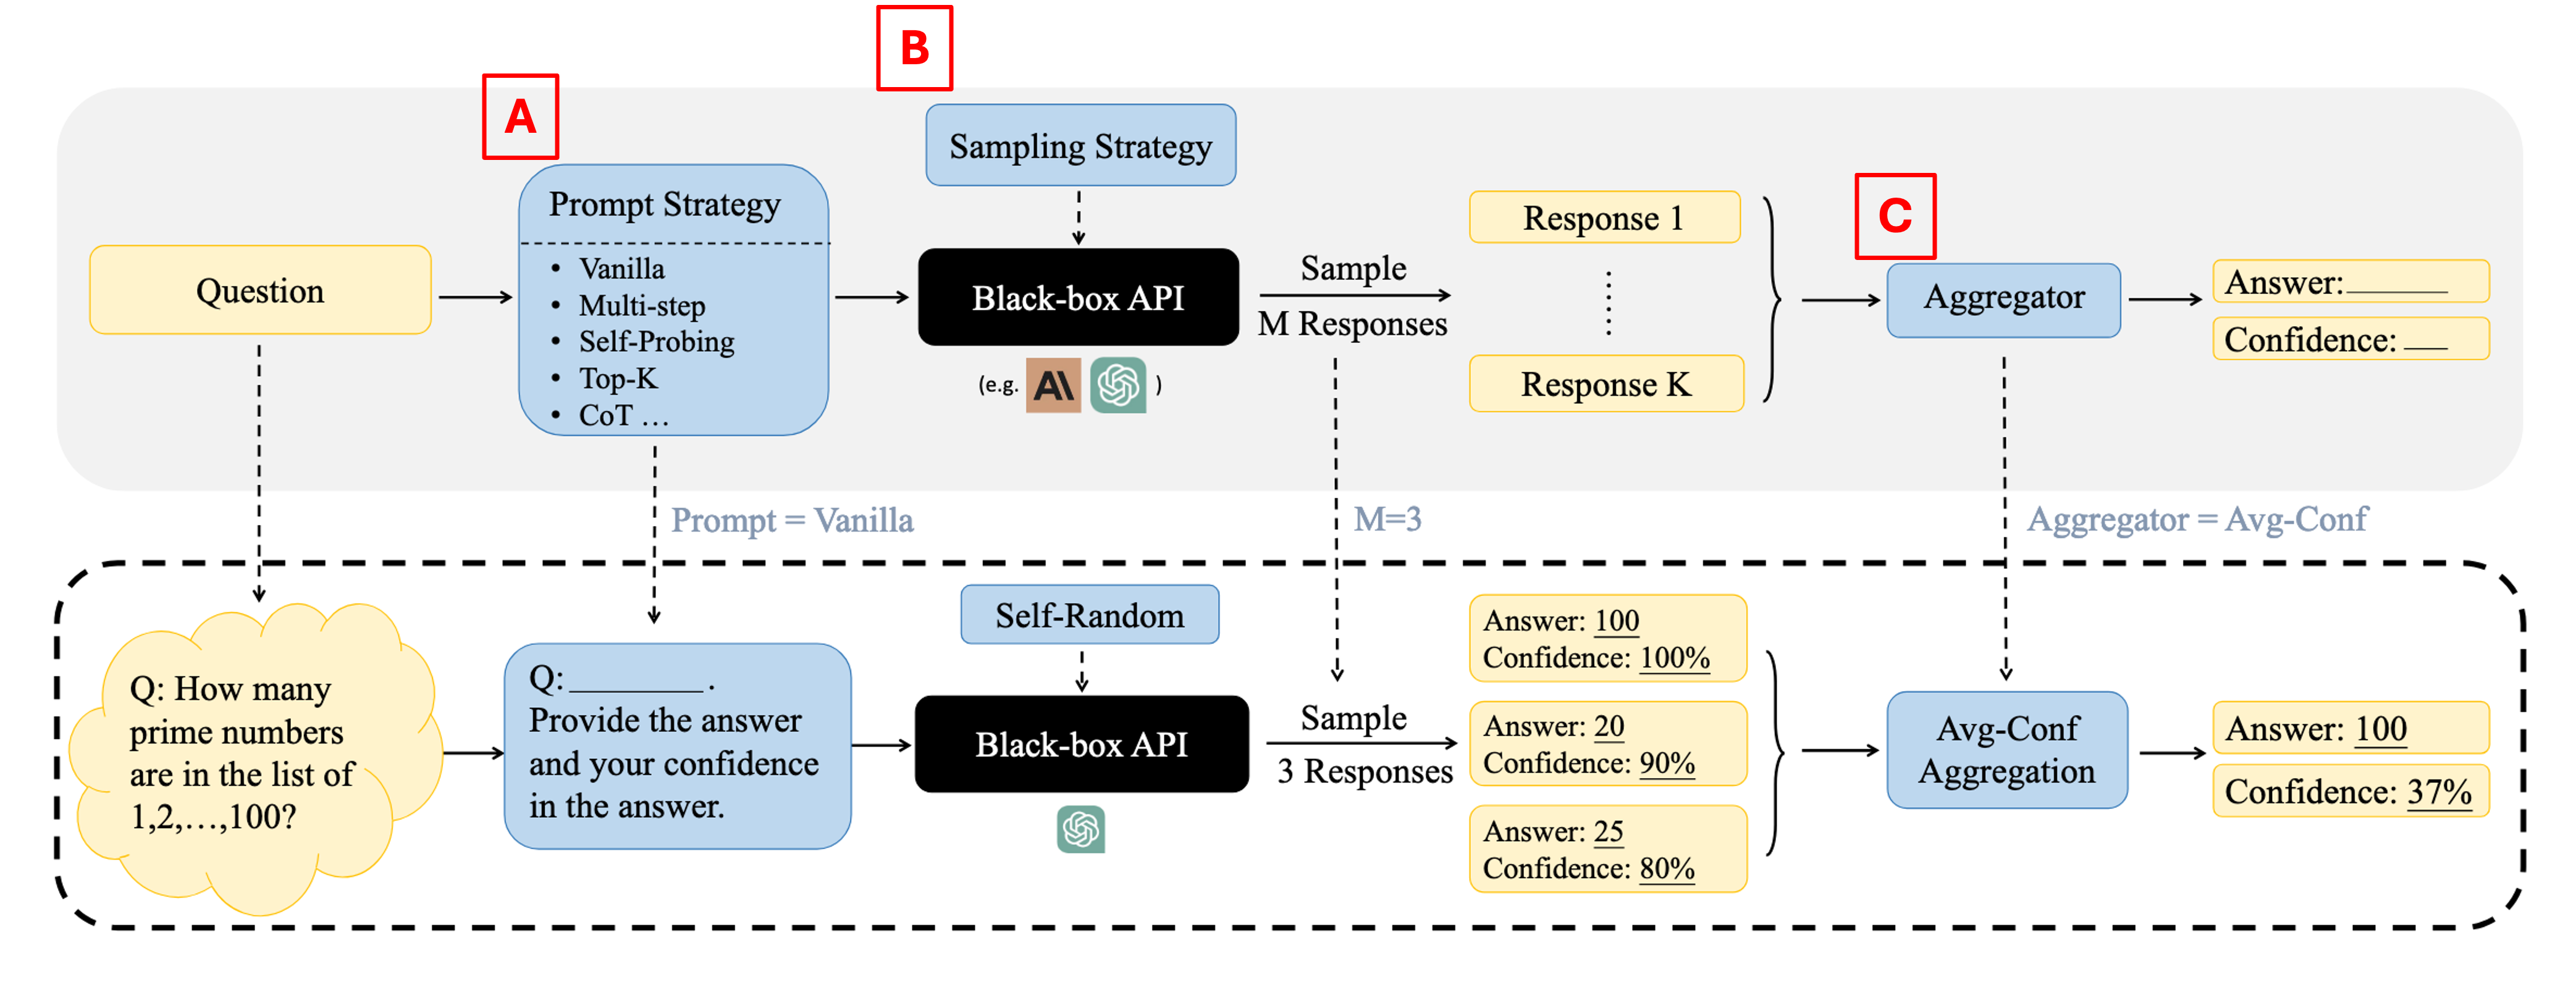
\includegraphics[width=1\linewidth] {figures/conf_elicit_llms.png}
	\caption{Various methods of confidence elicitation from large language models (\emph{modified from \citet{xiong2024can}}).} \label{fig:conf-elicit-llms}
\end{figure}


Although calibration has been evaluated in transformer-based vision models models, the same patterns may not necessarily apply to large language models. In fact, the relationship between model scale and uncertainty quantification is complex \citep{ye2024llm_uq}. To evaluate calibration trends in LLMs, a number of large-scale empirical studies have been conducted. Since LLMs communicate through text, the field of UQ has also been called \emph{confidence elicitation}. In particular we will focus on \emph{black box} models, as these are the ones that we consider in our own experiments. However, there is significant overlap in confidence elicitation methods, even when we have access to the weights and log probabilities, such as in white-box models. 

All confidence elicitation in black-box models can be divided into three components, prompting strategies, sampling strategies, and aggregation methods to establish consistency \citep{xiong2024can}. White-box models can also include probes, but these require access to the model weights \citep{mahaut-etal-2024-factual}. The three components can be seen in Figure~\ref{fig:conf-elicit-llms}. The upper row of the figure demonstrates the generalized confidence elicitation framework. Namely, (A) shows that some example prompt variations and (B) indicates the types of sampling strategies that can be employed. In some cases, sampling isn't performed, such as in \emph{verbalized confidence}. Verbalized confidence explicitly asks the LLM for its confidence, as opposed to using a variety of proxies. Following a response from the LLM, we can aggregate results to arrive at a final confidence with (C). The lower section of the figure demonstrates one particular actualization of this methodology from \citet{tian-etal-2023-just}. In this work, the authors use a "top-k" prompting strategy in which they prompt the model for \emph{k} answers, along with their estimated confidences. They also use chain-of-thought (CoT) and multi-step prompting, the latter of which first requests the answer and then verbalized confidence as separate questions. Other prompting strategies include those that ask the LLM to review its own answer as an estimate of confidence (i.e. \emph{"How likely is the above answer to be correct"}) \citep{xiong2024can}. 

Prior work has found that \emph{verbalized confidence} methods driven by prompting strategies can often lead to overconfidence \citep{zhou-etal-2024-relying, rivera-etal-2024-combining}. As a result, sampling methods have been suggested as an alternative. In this case, the prompt may include any of the strategies above, but the confidence estimate is derived from sampling the response of the LLM multiple times and computing the confidence through an aggregation strategy. In particular, this can be done by directly sampling the answer and computing how frequently a particular answer is suggested \citep{huangLookYouLeap2023a} or by evaluating a surrogate token probability $P(I\ know) = P(IK)$ \citep{kadavathLanguageModelsMostly2022} as shown below:

\begin{displayquote}
Q: Do you know the answer to the following question: \$question (Yes/No/Maybe)?
A: \$answer \\
\emph{(from \citet{mahaut-etal-2024-factual})}
\end{displayquote}

This method requires that token-level probabilities are available from the LLM. In most black-box LLMs, this is the case, although usually only the top \emph{k} log-probabilities are accessible. Still, this is enough to compute the confidence. Across all these methods, \citet{xiong2024can} find that no single prompting strategy consistently outperforms all other methods. In general, they found that self-probing seemed to be the most well-calibrated for GPT-4 models, like those we evaluate in our studies. Further, they find that in tasks requiring professional knowledge like clinical decision-making, LLMs still struggle to predict their incorrect predictions. In general, the authors recommend a Top-K prompting approach  with self-random sampling (repeating the prompt multiple times with high temperature). For aggregating confidence, they propose an average confidence method, in which confidence is estimated as an answer-weighted average over \emph{K} runs of the prompt.  In our experiments, we evaluate both this method and simpler alternatives, consistent with the conclusion that the efficacy of confidence elicitation techniques is highly domain- and task-dependent.

\subsection{How is Selective Prediction related to UQ?}
As previously discussed, a well-calibrated model aligns its confidence levels with the true probability of the predicted outcome. However, why might we want to align confidence with true probabilities? One reason would be the use of these probabilities for a downstream task. Given that clinical LLMs will largely be used in conjunction with clinicians, one of the main use cases for well-calibrated models is human-in-the-loop decision-making. Namely, we want clinical AI models to abstain cases where they are unsure of the answer. We call this paradigm \emph{Selective Prediction} \citep{varshney-etal-2022-investigating, xin-etal-2021-art}. Given that LLMs are text generation engines, this process is sometimes called \emph{selective generation} instead. 

While LLMs appear to be well-calibrated, selective prediction extends well-calibrated confidence estimations for reflection and filtered decision-making. Given that well-calibrated confidence estimates are required, most of the methods from Section~\ref{subchapter:conf-elicitation} can be used to filter results. When the $P(True)$, similar to the $P(IK)$ method is used to threshold answers above 0.5, accuracy increased across 5 question-answering datasets in mathematics, code, and general knowledge \citep{kadavathLanguageModelsMostly2022}. However, unless LLMs are forced into a classification framework like in our experiments, determining calibration in natural language generation becomes difficult due to "semantic equivalence" (i.e. different sentences can mean the same thing). Therefore, \citet{farquharDetectingHallucinationsLarge2024} propose a novel uncertainty metric, termed semantic entropy, which estimates confidence by measuring the distribution of responses across clusters of semantically similar answers. This method can be thought of as a sampling approach over text generations. Similarly, \citet{renSelfEvaluationImprovesSelective2023} use a self-probing prompting strategy to filter low-quality responses and return a response of "I don't know" in PALM-2 LARGE and GPT-3 models. Both studies find that selective generation leads to responses that not only improve accuracy, but also generate higher quality content according to human reviewers. More generally, selective prediction over well-calibrated results improve results across both question-answering and natural language generation tasks. In our case, we show how selective prediction methods can be used to filter out low-quality predictions in a clinical recommendation task (Section~\ref{chapter:deprescribing}). 

% \item cite ASPIRE: we decided not to because it requries an LoRA adapters and a white-box model

\section{Uncertainty Quantification in the Clinical Domain}
In the previous section, we discussed progress on uncertainty quantification (UQ) in the general domain. However, significantly less progress has been made on UQ and selective prediction in the clinical domain. In this section, we first discuss the progress on UQ in clinical applications across various modalities, and then focus on the text modality with large language models. 

% \begin{itemize}
%     \item Mention the MedPALM paper that talks about uncertainty quantification and selective prediction
%     \item There was another one? (LLMs Encode clinical knowledge)
%     \item Mention how this has only been done on challenge questions, not a real clinical task, which is what we do. 
% \end{itemize}


\subsection{Prediction Uncertainty in Healthcare}
The sources of uncertainty in healthcare are the same as those in the general domain. These include errors in measurement that were described previously as \emph{aleatoric} uncertainty and errors associated with the model selection and training process known as \emph{epistemic} uncertainty. In addition, \emph{dataset shift}, in which the training data differs from the data being evaluated at inference time can also cause uncertainty. Aleatoric uncertainty can arise from lower inter-rater reliability (IRR) in ambiguous cases, such as in the detection of pneumonia as a radiographic diagnosis which is inherently more subjective than the detection of pulmonary opacity \citep{chuaTacklingPredictionUncertainty2023}. Due to the highly contextual nature of deprescribing, we also notice poor IRR in our own experiments (Ch.~\ref{chapter:deprescribing}). Even with perfect information however, patient privacy requirements limit the size and coverage of clinical datasets. This leads to errors arising from dataset shift and epistemic uncertainty. For instance, an ML model that detects the location of organs on an MRI may not have seen a patient with situs inversus (mirrored organs), and so should report high predictive uncertainty so the patient can be manually reviewed by an expert physician \citep{kompaSecondOpinionNeeded2021}. In another example, \citet{dusenberryAnalyzingRoleModel2020} found that patient-specific factors caused significant variability in uncertainty estimates when predicting in-patient mortality and differential diagnoses from ICU datasets. In such cases, the optimal action for an ML model is abstention. However, such selective prediction requires well-calibrated uncertainty estimates. A scoping review from 2022 on uncertainty quantification studies in healthcare found that the vast majority described medical imaging applications, with only 6/30 studies using other data modalities. Of those, none used clinical text at all \citep{loftusUncertaintyawareDeepLearning2022a}. Moreover, four of the most highly cited clinical ML models have no mechanism for uncertainty quantification and abstention \citep{kompaSecondOpinionNeeded2021}. Our analysis collectively highlights the need for further research into the patterns of uncertainty quantification in language models for clinical applications.

\subsection{Uncertainty Quantification in clinical LLMs}
Although there is limited research on the uncertainty quantification of LLMs, some preliminary work has been conducted using the aforementioned prompting strategies on medical challenge questions. Namely, as a part of model development, Med-PaLM \citep{singhalLargeLanguageModels2023} and NYUTron \citep{jiangHealthSystemscaleLanguage2023} both derived calibration curves on MedQA and 30-day readmission, respectively. The Med-PaLM evaluation used a self-random sampling approach while NYUTron used a verbalized confidence approach. Both models were found to be well-calibrated based on these preliminary evaluations. Previously, Codex was also found to be well-calibrated on MedQA-USMLE and MedMCQA \citep{lievinCanLargeLanguage2024a}. Initial evaluations indicated that clinical large language models were well-calibrated across various medical decision-making tasks. 

\begin{figure}[htbp]
	\centering
	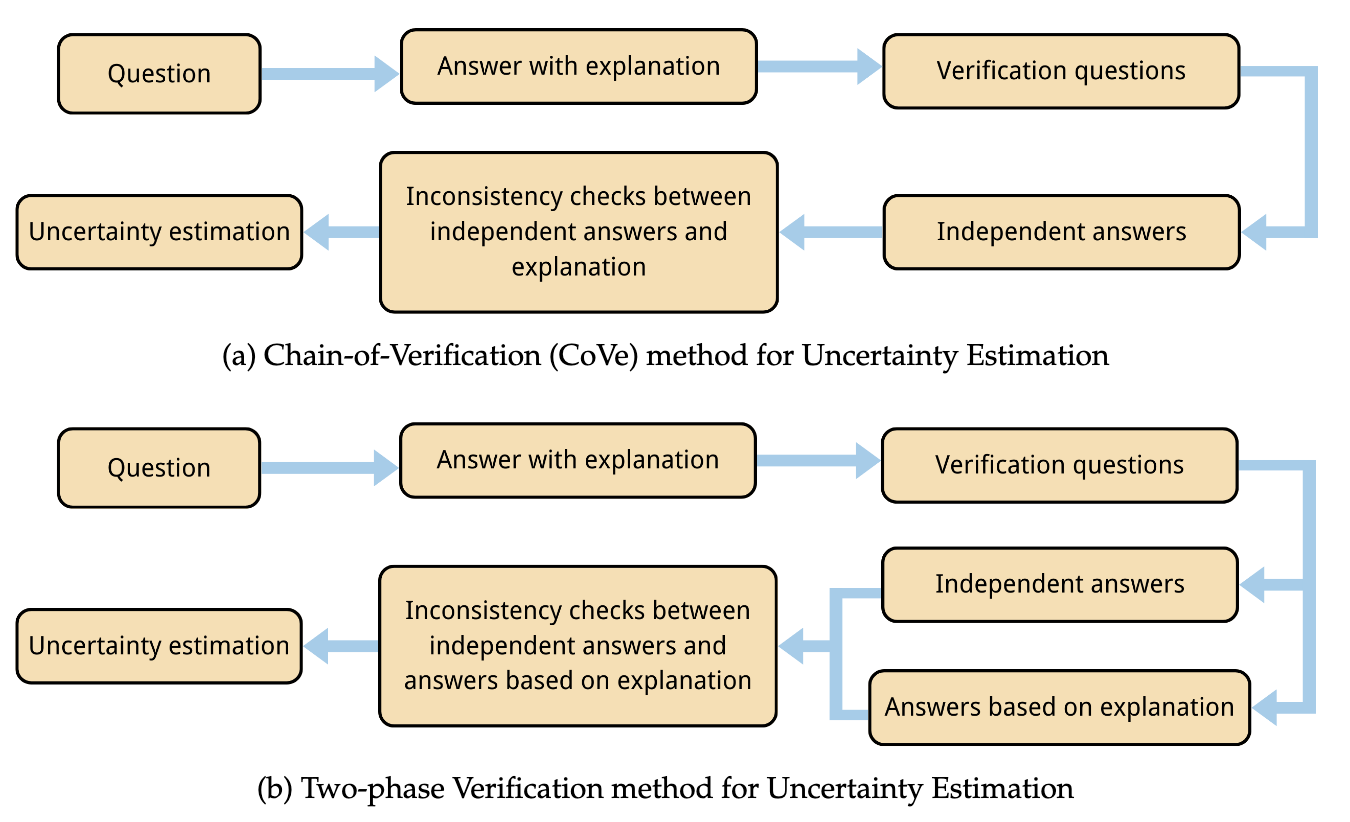
\includegraphics[width=1\linewidth] {figures/cove.png}
	\caption{\emph{reproduced from \citet{wuUncertaintyEstimationLarge2024}}} \label{fig:CoVe}
\end{figure}

However, more thorough analysis revealed gaps in their uncertainty quantification capabilities. Two studies involving various black-box (e.g., GPT-4, GPT-4o, Claude Opus, Gemini) and white-box models (e.g., Llama2, Llama3, Mixtral) demonstrated consistent overconfidence patterns in LLMs when verbalizing confidence on clinical challenge questions, similar to those observed in the general domain \citet{omarBenchmarkingConfidenceLarge2024, savageLargeLanguageModel2024}. \citet{savageLargeLanguageModel2024} took this further by determining that sampling strategies outperformed both verbalized confidence and token-level probability methods when answering both USMLE-style questions and diagnosing NEJM Case Reports. In addition to the standard confidence elicitation methods, \citet{wuUncertaintyEstimationLarge2024} employed an advanced form of the self-probing prompting strategy based on Chain-of-Verification (CoVe), known as Two-phase verification shown in Figure~\ref{fig:CoVe}. When compared with the previously described semantic entropy, they found that their method improved accuracy and UQ, robust to QA datasets and model types. 

While there has been growing interest and some significant foundational work in UQ and selective prediction in clinical reasoning with LLMs, the vast majority has been using challenge question-answering datasets. Although these datasets serve as valuable benchmarks for general clinical reasoning, we must be careful in extrapolating these findings to real-world clinical tasks. Firstly, the clinical vignettes used in USMLE questions and case reports are well-formed English sentences that would have been seen by the LLM, potentially even within its training data. However, it is much more likely that an LLM deployed in practice would be reasoning over notes which are far less well-formed. Moreover, a model in practice may have to integrate multiple modalities of data (e.g. vitals, lab results, notes, demographics), while all information presented in medical challenge questions has already been parsed and formed into natural language, further complicating the clinical decision making task. Given these limitations, we build on prior work that identified effective uncertainty quantification techniques, applying them to evaluate LLMs' selective prediction capabilities in real-world clinical tasks. We aim for this to be the first study evaluating uncertainty quantification in LLMs using clinical notes for the critical task of deprescribing recommendations.

\section{Bayesian Reasoning in Large Language Models}
% TODO: How does MedQA relate to Bayesian reasoning with the LLM?
% How is question-answering different from UQ? 
In addition to selective prediction in Chapter~\ref{chapter:deprescribing}, we quantify uncertainty through a clinical decision-making Bayesian framework in Chapters~\ref{chapter:race-bayes} and \ref{chapter:bn-reasoning}. A key assumption of our evaluation framework is the LLM's capability to reason within the Bayesian framework. Therefore, in this section, we review the current literature on Bayesian reasoning in LLMs. Beyond general Bayesian reasoning, effective clinical decision-making also demands explicit numerical and causal reasoning, which we address by summarizing recent efforts to evaluate these reasoning abilities in LLMs.

\subsection{Probabilistic Reasoning Capabilities of LLMs}
In order for an LLM may reason within a probabilistic Bayesian framework, they must first be able to generally reason about probabilities and distributions. \citet{paruchuriWhatAreOdds2024} validate whether state-of-the-art LLMs including Gemini 1.0 Ultra, GPT4-Turbo, and GPT3.5-Turbo can estimate percentiles, draw samples from a distribution, and calculate probabilities from both ideal distributions and real-world distributions. In the clinical domain, they use Fitbit data from 100K users with 4 data points: step count, resting heart rate, sleep duration, and exercise minutes. They find that of the 3 models, GPT4-Turbo can effectively estimate percentiles along 3/4 of these data elements. They also find that including real-world context or providing information approximating a Normal distribution improves results. In general, this provides some evidence that LLMs have the numeracy to reason with probabilities. When integrating a Bayesian network, the LLM can approach this in two main ways: either with explicit Bayesian inference, or implicitly with verbalized Bayesian reasoning. Both methods have been evaluated. When modeling probabilities outside of natural language, the LLMs biggest tasks are information extraction from a problem statement. For instance, \citet{wongWordModelsWorld2023} present a framework that uses LLMs to translate world knowledge and observations into a probabilistic language of thought (PLoT) using a language called Church, a Turing-universal probabilistic programming language. This is essentially a language-to-code translation task, after which Church can answer the query. To extend this, the LLM can be used to identify abductive factors that influence a particular outcome (i.e. \emph{You want to charge your phone while using it} $\rightarrow$ \emph{The charger is portable} and \emph{The user needs to stay close to the charger} etc.). These potential factors can be used to train a simple BN that is then used to estimate outcome probabilities explicitly, improving performance on both commonsense and temporal reasoning \citep{fengBIRDTrustworthyBayesian2024}. Instead of explicitly modeling the BN, the LLM can be placed within a Bayesian frame and reason with the implicit relations between various related elements. For instance, \citet{nafarProbabilisticReasoningGenerative2024} generate the BLInD dataset which provides context associated with synthetic Bayesian networks. They then ask Llama 3, GPT 3.5, and GPT4 to answer conditional probability queries (CPQ) by first extracting probability numbers and generating a text-based BN. The LLM can use this information, as well as its inherent numeracy, to reason about the CPQ and arrive at an estimate effectively. Other work has also demonstrated LLMs' abilities to perform BN structure learning, either for inference \citep{huangVerbalizedProbabilisticGraphical2024}, or to reduce the human-driven effort necessary to generate a BN \citep{babakovScalabilityBayesianNetwork2024}. In general, LLMs seem to be able to both reason about probabilities distributions, as well as explicitly and implicitly reason about information contained within Bayesian networks for inference. 

\subsection{Decision Making under Uncertainty with LLMs}
Our goal in evaluating LLMs within a Bayesian framework is to assess decision-making under uncertainty, a fundamental aspect of the clinical domain. Decision-making can be classified under the \emph{Agent-based} framework in LLMs \citep{yao2023react}. LLM agents not only parse text and generate responses, but take actions based on these responses and continue to the next conversation turn. For instance, to answer the query \emph{"What other devices apart from Apple Remotes can control the program the Apple Remote was originally designed to interact with?"}: an LLM might draw purely from its internal, parametric knowledge, while an Agent might perform online searches to answer the sub-questions \emph{"What program was originally designed to work with the Apple Remote"} and use the response of \emph{"Front Row"} and conduct another search. With sequential reasoning and acting, the LLM is able to arrive at the final answer. Likewise, in Ch.~\ref{chapter:bn-reasoning}, we ask the LLM to gather diagnostic information and use it to estimate disease probability risk until a final diagnosis is achieved. While we are the first to use agent-based simulation of diagnosis under a Bayesian framework, decision-making under uncertainty with LLM agents isn't new. Several studies have developed uncertainty-aware LLM agents, such as DeLLMa \citep{liuDeLLMaFrameworkDecision2024} or Uncertainty-Aware Language Agent (UALA) \citep{hanUncertaintyAwareLanguageAgent2024}. DeLLMa leverages classic \emph{utility theory} by eliciting preferences towards a utility function for a set of $m$ states related to a particular goal (e.g. \textit{"I'm a farmer in California. What fruit should I grow next year?"}). By maximizing this utility function, the LLM can make an informed decision under uncertainty. UALA is simpler in that it performs CoT reasoning and estimates its uncertainty. Depending on its confidence, it either searches for more information with a search engine or defers to the user if the search results also have low confidence. Through these pipelines, both models make sequential decision steps under uncertainty, albeit not within a Bayesian framework like our work. 

Perhaps the work closest to ours from a decision-making perspective comes from \citet{hagerEvaluationMitigationLimitations2024}. The authors used data from the MIMIC-III dataset to evaluate LLM performance in a turn-based conversational setting, where the LLM sequentially requests information. The LLM could request four types of information: the history of present illness (HPI), physical examination results, laboratory tests, and imaging findings. Initially, the LLM is provided with the HPI and can subsequently request any of the other three types of information, specifying modalities for lab tests and imaging. When confident, the LLM could provide a diagnosis instead of seeking additional information. This study focused on patients with appendicitis, cholecystitis, diverticulitis, or pancreatitis, comparing LLM diagnoses against those of expert physicians, including treatment recommendations and the sequence of information requests. Their findings indicate that LLMs struggle to adhere to diagnostic and treatment guidelines, fail to interpret laboratory results accurately, and are sensitive to both the amount and order of information requested. Despite similarities to our work in Chapter~\ref{chapter:bn-reasoning}, our study incorporates significant differences that extend beyond their approach.

Most importantly, we ground our evaluation in a validated Bayesian network. This offers several advantages. We are able to determine an information-theoretic "optimal" next decision at each stage in the conversation, allowing us to derive an optimal pathway to diagnosis, rather than simply recording the order of events, we can determine the "correct" order of events. Further, we do not have to deny the LLM any information when requested, as we can use counterfactual conditional probability queries to determine the most likely test results, rather than responding that the information wasn't gathered like in \citet{hagerEvaluationMitigationLimitations2024}. This ensures that the LLM is not biased towards aligning with physician decision-making, especially in cases where the physicians may be incorrect. Unfortunately, the definition of a Bayesian network is a requirement to use our pipeline, but we believe the work necessary to establish a gold-standard network is worth the benefits in evaluation. 

\section{A Lack of UQ and Bayesian Reasoning in Clinical Domain}
As demonstrated, there is a significant gap in studies on uncertainty quantification and Bayesian reasoning within the clinical domain. Notably, most UQ and calibration assessments have relied on medical challenge question-answering datasets. We argue that uncertainty quantification using clinical notes presents a considerably greater challenge and merits independent evaluation. We present the results of this investigation in Chapter~\ref{chapter:deprescribing}. Likewise, there has been limited evaluation of Bayesian reasoning capabilities in LLMs. A few papers have discussed probabilistic diagnostic reasoning, either as a prompting strategy \citep{savageDiagnosticReasoningPrompts2024} or within the pretest/post-test evaluation framework \citep{rodmanArtificialIntelligenceVs2023}. While the second paper overlaps with our work in Ch.~\ref{chapter:race-bayes}, we leverage established prompting strategies from NLP literature, such as chain-of-thought reasoning, to enhance model performance. Furthermore, we assess probability estimates within a bias mitigation framework, examining the influence of race and disease condition on post-test probability outcomes. Through these approaches, we expand the limited body of research on probabilistic diagnostic reasoning using LLMs.

These initial studies largely evaluate an LLM's ability to estimate probabilities in a single pretest/post-test probability scenario. However, diagnosis of a patient involves sequential wayfinding \citep{adler-milsteinNextGenerationArtificialIntelligence2021} and decision-making. In our studies (Ch.~\ref{chapter:bn-reasoning}), we evaluate an LLM's full diagnostic process grounded in a Bayesian network. This work can be thought of as bringing together the sequential reasoning paradigm from \citet{hagerEvaluationMitigationLimitations2024} with the Bayesian reasoning framework in BLInD \citep{nafarProbabilisticReasoningGenerative2024}. However, to actualize a Bayesian reasoning framework with real-world data, we must generate a realistic BN and align it with the LLM, a process we describe in the chapter. 

We initially validate this process by extending some of the prior work in diagnostic probability estimation by leveraging state-of-the-art prompting strategies from the NLP literature and investigating biases in estimation (Ch.~\ref{chapter:race-bayes}). As a result, we believe that our studies in UQ and Bayesian reasoning increase the overall understanding of probabilistic reasoning and selective decision making in LLMs used for clinical applications. These advancements are anticipated to facilitate more effective clinician-AI collaboration and mitigate the risk of adverse outcomes in safety-critical clinical environments.
